% \documentclass[aip,jcp,preprint,unsortedaddress,a4paper,onecolum]{revtex4-1}
\documentclass[aip,jcp,a4paper,reprint,onecolumn]{revtex4-1}
% \documentclass[aps,pre,twocolumn]{revtex4-1}
% \documentclass[aps,jcp,groupedaddress,twocolumn,unsortedaddress]{revtex4}

\usepackage[fleqn]{amsmath}
\usepackage{amssymb}
\usepackage[dvips]{graphicx}
\usepackage{color}
\usepackage{tabularx}
\usepackage{algorithm}
\usepackage{algorithmic}

\makeatletter
\makeatother

\newcommand{\recheck}[1]{{\color{red} #1}}
\newcommand{\redc}[1]{{\color{red} #1}}
\newcommand{\bluec}[1]{{\color{blue} #1}}
\newcommand{\vect}[1]{\textbf{\textit{#1}}}
\newcommand{\dd}{\textsf{d}}
\newcommand{\inv}{\textrm{inv}}

\newcommand{\mh}{\mathcal H}
\newcommand{\ml}{\mathcal L}
\newcommand{\mt}{\mathcal T}
\newcommand{\mo}{\mathcal O}
\newcommand{\mi}{\mathcal I}
\newcommand{\mc}{\mathcal C}
\newcommand{\proj}{\mathit\Pi}
\newcommand{\fwg}{{\mathcal A}}
\newcommand{\bwg}{{\mathcal B}}
\newcommand{\bsigma}{\boldsymbol\sigma}


\begin{document}

\title{Linear response theory for core set identification}
\author{Han Wang}
% \affiliation{Institute for Mathematics, Freie Universit\"at Berlin, Germany}
\author{Christof Sch\"utte}
\affiliation{Institute for Mathematics, Freie Universit\"at Berlin, Germany}
% \affiliation{Institute for Mathematics, Freie Universit\"at Berlin, Germany}

\date{\today}

\begin{abstract}
  % In this draft, we are trying to study the core set based Markov
  % State Model (MSM) under non-equilirbium conditions.
\end{abstract}

\maketitle

\section{Theoretical background}
\subsection{Classical linear response theory}


In this section, we want to firstly give a brief description of the classical linear response
theory, for details see Ref.~\cite{tuckeman2010statistical} for
example.
In this paper we want to study the non-equilibrium system driven by some external force.
More strictly, we investigate the system that is governed by the
following Langevin equation:
\begin{align}\label{eqn:langevin-1}
  \dot{\vect q} & = \nabla_{\vect p}\mh(\vect q,\vect p), \\\label{eqn:langevin-2}
  \dot{\vect p} & =- \nabla_{\vect q}\mh(\vect q,\vect p)
  + \vect D(\vect q,\vect p) F_e(t)
  - \gamma\vect p
  + \sigma\dot{\vect W}.
\end{align}
Here $\vect D$ is the external driving force applied to the system, and
$F_e(t)$ is the strength of the driving as a function of time.
We always assume that the magnitude of $\vect D$ is controllable, and
the magnitude of $F_e(t)$ is small and of order $\mo (\varepsilon)$, $\varepsilon \ll 1$.
The phase space incompressibility condition is assumed:
\begin{align}
  \nabla_{\vect p}\cdot\vect D = 0
\end{align}
Then the phase space distribution $f(\vect x, t)$ ($\vect x = \{\vect
q, \vect p\}$) is subject to the Kolmogorov forward equation:
\begin{align}\label{eqn:orig-forward}
  \frac{\partial}{\partial t} f(\vect x, t) - \fwg^\beta(t) f(\vect x, t) = 0
\end{align}
where $\fwg^\beta(t)$ is the forward infiniesimal generator given by
\begin{align}
  \fwg^\beta(t) =
  \frac{\sigma^2}2\Delta_{\vect p}
  - \Big(
  \nabla_{\vect p}\mh + \vect C F_e(t)
  \Big)\cdot\nabla_{\vect q}
  - \Big(
  -\nabla_{\vect q}\mh +
  \vect D F_e(t) - \gamma\vect p
  \Big)\cdot\nabla_{\vect p}
  + 3N\gamma,
\end{align}
and $\beta$ is the inverse temperature.
The fluctuation-dissipation relation is always true:
$\beta = 2\gamma / \sigma^2$.
The equilibrium and non-equilibrium system
is governed by
the standard Langevin equation, i.e. with
vanishing driving force $F_e(t) = 0$ in
Eqn.~\eqref{eqn:langevin-1} and \eqref{eqn:langevin-2}.
We assume that the driving to the
system is so small that both the phase space distribution and the
infiniesimal generator can be viewed as perturbation from the initial
distribution and the un-driven generator
($\vect D = 0$),
respectively. We the expansion with respect to small
variable $\varepsilon$:
\begin{align}\label{eqn:f-expan}
  f(\vect x, t) &= f_0(\vect x, t) + \varepsilon f_1(\vect x, t)
  +\varepsilon^2 f_2(\vect x, t) + \mo (\varepsilon^3),
\end{align}
and 
\begin{align}\label{eqn:A-expan}
  \fwg^\beta(t) = \fwg^\beta_0 + \varepsilon\fwg_1(t),
\end{align}
where
\begin{align}
  \fwg_0^\beta =&
  \frac{\sigma^2}2\Delta_{\vect p}
  -
  \nabla_{\vect p}\mh\cdot\nabla_{\vect q}
  - \big(
  -\nabla_{\vect q}\mh - \gamma\vect p
  \big)\cdot\nabla_{\vect p}
  + 3N\gamma,\\
  \fwg_1(t) =&
  - \frac{F_e(t)}{\varepsilon} \big(
  \vect C \cdot\nabla_{\vect q}
  +
  \vect D \cdot\nabla_{\vect p}
  \big).
\end{align}
Notice $F_e(t) \sim \mo(\varepsilon)$, so $\Vert\fwg_1(t)\Vert\sim\mo(1)$.
The invariant measure of $\fwg^\beta_0$ satisfies $\fwg^\beta_0f^\beta_{\inv}(\vect x) = 0$,
which is nothing but the Boltzmann distribution
\begin{align}
  f^\beta_{\inv}(\vect x) \propto e^{-\beta\mh(\vect x)}
\end{align}
Inserting \eqref{eqn:f-expan} and \eqref{eqn:A-expan} into
\eqref{eqn:orig-forward}, 
the Kolmogorov forward equation becomes:
\begin{align}
  \frac{\partial}{\partial t}
  [f_0(\vect x, t) + \varepsilon  f_1(\vect x, t) + \varepsilon^2f_2(\vect x, t)]
  -
  [\,\fwg^\beta_0 + \varepsilon\fwg_1(t)\,]
  [f_0(\vect x, t) + \varepsilon  f_1(\vect x, t) + \varepsilon^2f_2(\vect x, t)]
  = 0
\end{align}
Matching this equation at different orders of $\varepsilon$, the zeroth
order gives:
\begin{align}\label{eqn:e-o0}
  \bigg[
  \frac{\partial}{\partial t}
  - \fwg_0^\beta
  \bigg]
  f_0(\vect x, t)
  = 0
\end{align}
which is the un-driven equation. Matching the first and the second order gives:
\begin{align}\label{eqn:e-o1}
  \bigg[
  \frac{\partial}{\partial t}
  - \fwg_0^\beta
  \bigg]
  f_1(\vect x, t)
  =&
  \fwg_1(t) f_0(\vect x, t)\\\label{eqn:e-o2}
  \bigg[
  \frac{\partial}{\partial t}
  - \fwg_0^\beta
  \bigg]
  f_2(\vect x, t)
  =&
  \fwg_1(t) f_1(\vect x, t)
\end{align}
Formally solving \eqref{eqn:e-o0} -- \eqref{eqn:e-o2} with
initial conditions $f_1(\vect x, 0) = 0$ and $f_2(\vect x, 0) = 0$
gives
\begin{align}\label{eqn:f0-0}
  f_0(\vect x, t)
  =&\,
  e^{t\fwg^\beta_0}f_0(\vect x, 0) \\\label{eqn:f1-0}
  f_1(\vect x, t)
  =&\,
  \int_0^t\dd s\,
  e^{(t-s)\fwg^\beta_0}\circ
  \fwg_1(s) f_0(\vect x,s)
  =
  \int_0^t\dd s\,
  e^{(t-s)\fwg^\beta_0}\circ
  \fwg_1(s)\circ
  e^{s\fwg^\beta_0}f_0(\vect x, 0) \\\nonumber
  f_2(\vect x, t)
  =&\,
  \int_0^t\dd s\,
  e^{(t-s)\fwg^\beta_0}\circ
  \fwg_1(s) f_1(\vect x,s) \\\label{eqn:f2-0}
  &=
  \int_0^t\dd s
  \int_0^s\dd u\,\,
  e^{(t-s)\fwg^\beta_0}\circ
  \fwg_1(s)\circ
  e^{(s-u)\fwg^\beta_0}\circ
  \fwg_1(u)\circ
  e^{u\fwg^\beta_0}
  f_0(\vect x, 0) 
\end{align}
If the initial distribution is the invariant distribution, i.e.
$f_0(\vect x, 0) = f_{\inv}^\beta(\vect x)$,
\eqref{eqn:f0-0} becomes:
\begin{align}
  f_0(\vect x, t) = f_{\inv}^\beta(\vect x)
\end{align}
It can be shown that
\begin{align}
  \fwg_1(s) f_{\inv}^\beta(\vect x)
  =
  -\frac{F_e(s)}{\varepsilon}\beta
  j(\vect x)
  f_{\inv}^\beta(\vect x),
\end{align}
where the \emph{dissipative flux} $j(\vect x)$ is defined by,
\begin{align}
  j(\vect x) =
  -\vect C\cdot\nabla_{\vect q}\mh 
  -\vect D\cdot\nabla_{\vect p}\mh
\end{align}
Then $f_1(\vect x, t)$ becomes:
\begin{align}
  f_1(\vect x, t)
  =
  -\frac\beta\varepsilon
  \int_0^t\dd s\,
  F_e(s)\,
  e^{(t-s)\fwg^\beta_0}
  \big[
  j(\vect x)
  f_{\inv}^\beta(\vect x)
  \big]
\end{align}
Therefore, the linear order approximation to
the solution of~\eqref{eqn:orig-forward} is 
\begin{align}\label{eqn:solv-orig-linear}
  f(\vect x, t) =
  f_{\inv}^\beta(\vect x)
  - \beta
  \int_0^t\dd s\,
  F_e(s)\,
  e^{(t-s)\fwg^\beta_0}
  \big[
  j(\vect x)
  f_{\inv}^\beta(\vect x)
  \big]
  + \mo(\varepsilon^2)
\end{align}
For any time-dependent observation, the linear response approximation
would be:
\begin{align}\nonumber
  \mathcal O(t)
  &=
  \int\dd \vect x \:O(\vect x)f(\vect x, t)  \\\nonumber
  &=
  \int\dd \vect x\, O(\vect x)\,
  [\,f_{\inv}^\beta(\vect x) + \varepsilon f_1(\vect x, t)] \\\nonumber
  &=
  \langle O\rangle
  -
  \beta
  \int \dd \vect x\:
  O(\vect x)
  \int_0^t\dd s\,F_e(s)
  e^{(t-s)\fwg_0^\beta}
  \big[j(\vect x)f^\beta_{\inv}(\vect x)\big]
  \\\nonumber
  &=
  \langle O\rangle
  -
  \beta
  \int_0^t\dd s\,
  F_e(s)
  \int \dd \vect x\,
  O(\vect x)\,
  e^{(t-s)\fwg_0^\beta}
  \big[j(\vect x)f^\beta_{\inv}(\vect x)\big]
  \\\nonumber
  &=
  \langle O\rangle
  -
  \beta
  \int_0^t\dd s\,
  F_e(s)
  \int \dd \vect x\,
  f^\beta_{\inv}(\vect x) j(\vect x)\,
  e^{(t-s)\bwg^\beta_0}
  O(\vect x)\\ \label{eqn:eqi-pert-1}
  &=
  \langle O\rangle
  -
  \beta
  \int_0^t\dd s\,
  F_e(t-s)
  \int \dd \vect x\,
  f^\beta_{\inv}(\vect x) j(\vect x)\,
  e^{s\bwg_0^\beta}
  O(\vect x)
\end{align}
Where $\bwg^\beta_0$ is the infiniesimal generator of the \emph{un-driven} 
Kolmogorov backward equation, which is the adjoint operator of $\fwg^\beta_0$.
We have
\begin{align}
  e^{s\bwg^\beta_0} O(\vect x) = \mathbb E_{\vect x} [O(\vect X^\beta_s)]
\end{align}
where $\vect X^\beta_t$ is the trajectory of the un-driven Langevin equation
starting at $\vect x$.
Therefore, we have
% Notice that $e^{i\ml_0(t-s)}O(\vect x) = O(\phi_{t-s}(\vect x))$,
% where $\phi_t(\vect x)$ is the flow mapping of the \emph{unperturbed}
% Hamiltonian system. We have
\begin{align}
  \mathcal O(t)
  =
  \langle O\rangle
  -
  \beta
  \int_0^t\dd s\,
  F_e(t-s)
  \int \dd \vect x\,
  f^\beta_{\inv}(\vect x)
  j(\vect x)\,
  \mathbb E_{\vect x} [O(\vect X^\beta_s)]
\end{align}
or equivalently:
\begin{align}\label{eqn:lr}
  \mathcal O(t)
  =
  \langle O\rangle
  -
  \beta
  \int_0^t\dd s\,
  F_e(t-s)
  \big\langle
  j(0)\,
  \mathbb E_{\vect x} [O(\vect X^\beta_s)]
  \big\rangle
\end{align}
where $  \langle
  j(0)\,
  \mathbb E_{\vect x} [O(\vect X^\beta_s)]
  \rangle$ is the \emph{equilibrium time
  correlation} between the observation $O$ at time $s$ and the
dissipative flux $j$.



\subsection{The non-equilibrium response theory}

The classical response theory mainly has the following two limitations:
Firstly, one has to start from an equilibrium simulation. That means if the
external driving is no longer small ($\varepsilon$ is relatively big), the
first order (or linear) response~\eqref{eqn:lr} may not be a good approximation to
the true non-equilibrium process any more.
One possible way to improve the accuracy is to introduce the second
order response term, i.e.~\eqref{eqn:f2-0}.
Here one encounters the second limitation of the classical
response theory: it does not provide a frame work, under which
the second and even higher order responses can be easily derived.
The limitations of the classical responses theory motivate us to
develop a more general frame work that allows one starting from any
non-equilibrium process (arbitrarily driven), and calculating from it as many orders of
responses as necessary.

In the language of path integral, the time-dependent average $O( t)$
can be written as
\begin{align}
  O( t) =
  \langle O[\vect X_s]\,\rangle_{0,t} = 
  \int\dd \vect u\, f(\vect u, 0) 
  \int_{\mc\{\vect u,0; t\}}
  O[\vect X_s]\, \dd\mathcal P[\vect X_s]  
\end{align}
where $O[\vect X_s]$ is the observable of the trajectories, which is a generalization of the
observable that only depends on the configuration of the system.
$\langle \cdot \,\rangle_{0,t}$ is the ensemble average over all possible trajectories in time interval $[0,t]$.
$f(\vect x, 0)$ is the initial distribution that may not be the equilibrium distribution.
$\mc\{\vect u,0; t\}$ is the set of all continuous trajectories starting from point
$\vect u$ at time $0$, and ending at some position at time $t$.
$\mathcal P[\vect X_s]$ is the
probability measure of the trajectories generated by driven Langevin dynamics~\eqref{eqn:langevin-1}--\eqref{eqn:langevin-2},
where the intensity $F_e$ need not to be 0.
Now we want to consider a system that is a small perturbation of the previous system (we now call it ``reference system'')
in the sense that it has a similar driven force: $F_e + \Delta F_e$, where $\Delta F_e\sim \mo(\varepsilon)$ is small.
The probability measure of the trajectories of this perturbed system is denoted by
$\tilde{\mathcal P}[\vect X_s]$.
The time-dependent average of observable of the system $F_e + \Delta F_e$ can be written down in terms of
the probability measure of the reference system:
\begin{align}
  \tilde O(t) =
  \int \dd\vect u f(\vect x,0)
  \int_{\mc\{\vect u,0; t\}} O[\vect X_s]\,
  \frac{\dd\tilde{\mathcal P}[\vect X_s]}{\dd\mathcal P[\vect X_s]}
  \, \dd\mathcal P[\vect X_s]    
\end{align}
by using the Girsanov formula, 
\begin{align}\label{eqn:girsanov}
  \frac
  {\dd\tilde{\mathcal P}[\vect X_s]}
  {\dd\mathcal P[\vect X_s]}  
  =&\,
  \exp
  \big\{{G[\vect X_s] - \frac12 H[\vect X_s]}
  \big\}
\end{align}
where the short notations are defined by:
\begin{align}
  G[\vect X_s]
  &= \frac{1}\sigma\int_0^t
  \Delta F_e(s)\,\vect D(\vect q_s,\vect p_s)\cdot\dd\vect W_s \\
  H[\vect X_s]
  &=
  \frac 1{2\sigma^2}\int_0^t
  \Delta F_e^2(s)\,\vect D^2(\vect q_s,\vect p_s)\,\dd s
\end{align}
If the difference $\Delta F_e(t)$ is of order $\mo (\varepsilon)$, then $G[\vect X_s] \sim \varepsilon$ is
the first order term, and $H[\vect X_s] \sim \varepsilon^2$  is the second order term.
Then with the Taylor expansion of the right-hand-side of Eq.~\eqref{eqn:girsanov}, we have
\begin{align}\label{eqn:neq-response}
  \tilde O(t) -
  O(t)
  =
  \big\langle O[\vect X_s]\cdot G[\vect X_s]\big\rangle_{0,t}
  +
  \frac12 \big\langle O[\vect X_s] \cdot (G^2[\vect X_s] - H[\vect X_s] )\big\rangle_{0,t}
  +
  \mo (\varepsilon^3)
\end{align}
Here are some remarks of the main result Eq.~\eqref{eqn:neq-response}:
\begin{itemize}
\item The first term on the right-hand-side of Eq.~\eqref{eqn:neq-response} is the linear
  response of the reference non-equilibrium process (driven by $F_e$). The second term is the second order
  response. One can easily write down higher orders of response by the Taylor expansion
  of the right-hand-side of Eq.~\eqref{eqn:girsanov}.
\item When the observable $O[\vect X_s]$ only depends on the end point of the trajectory, i.e.
  $O[\vect X_s] = O(\vect X_t)$, then $\big\langle O(\vect X_t)\cdot G[\vect X_s]\big\rangle_{0,t}$
  gives the well-know time correlation form of the linear response.
\item If one wants to calculate a large amount of different perturbations, then apply one by one
  Eq.~\eqref{eqn:neq-response} is not convenient, because one has to calculate the responses
  again when the function form of $\Delta F_e$ is not a linear combination of previously calculated perturbations.
  If it is possible to
  express different $\Delta F_e$ by a group of base functions, then the responses are only need
  to calculated on the bases. Then with a linear conbination of the responses on bases, one can derive
  the responses of the whole group of perturbations. 
\item In the prove, we assume that the reference and the perturbed non-equilibrium processes
  have the same initial distribution (both of them may be different from the equilibrium distribution),
  but this is not a necessary. One can easily
  applies similar perturbation approach to the initial distribution as  to the trajectory ensemble.
  To keep the story simple, we do not develop the theory from this aspect.
\end{itemize}














\section{Numerical tests}

\subsection{The tilting double-well potential}

\begin{figure}
  \centering
  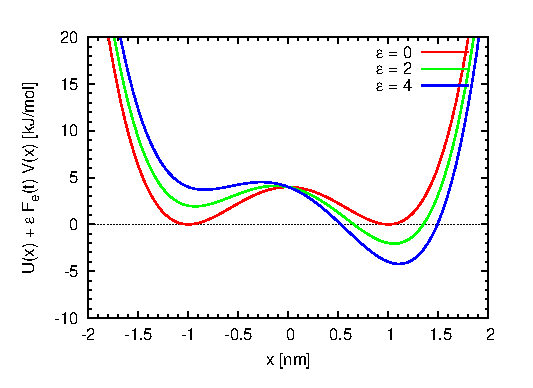
\includegraphics[width=0.4\textwidth]{figs/fig-tilt-pot.eps}
  \caption{The double-well potential with tilting perturbation.}
  \label{fig:tmp1}
\end{figure}

\begin{figure}
  \centering
  \includegraphics[width=0.95\textwidth]
  {figs/fig-tilt-str2-2d-more.eps}
  \caption{The plot of $\Delta\mt_\tau f(\vect x,t)$  under perturbation of
    $F_e^{\textrm{max}} = 2$.
    The 1st row: the direct non-equilibrium
    simulation. The 2nd row: the results of linear response
    formula~\eqref{eqn:core-identify-approx-2}.
    The 3rd row: the results of response
    formula~\eqref{eqn:pert-approx-1} and \eqref{eqn:pert-approx-2}.
    The order is 2, the reference state is $F_e^{\textrm{max}} = 0$, i.e.
    the equilibrium state.
  }
  \label{fig:tmp2}
\end{figure}

\begin{figure}
  \centering
  \includegraphics[width=0.95\textwidth]
  {figs/fig-tilt-str4-2d-more.eps}
  \caption{The plot of $\Delta\mt_\tau f(\vect x,t)$  under perturbation of
    $F_e^{\textrm{max}} = 4$.
    The 1st row: the direct non-equilibrium
    simulation. The 2nd row: the results of linear response
    formula~\eqref{eqn:core-identify-approx-2}.
    The 3rd row: the results of response
    formula~\eqref{eqn:pert-approx-1} and \eqref{eqn:pert-approx-2}.
    The order is 2, the reference state is $F_e^{\textrm{max}} = 0$, i.e.
    the equilibrium state.
    The 4th row: the results of response
    formula~\eqref{eqn:pert-approx-1} and \eqref{eqn:pert-approx-2}.
    The order is 1, the reference state is $F_e^{\textrm{max}} = 2$.
  }
  \label{fig:tmp3}
\end{figure}

We test the idea firstly by a one-dimensional model system: one particle in a
tilting double-well potential. For convenience, we let the mass of the
particle to be 1 \textsf{amu}. The unperturbed
Hamiltonian of the system is given by:
\begin{align}
  \mh (\vect p, \vect q) = \frac 12 \vect p^2 + U(\vect q) 
\end{align}
with potential
\begin{align}
  U(\vect q) = \frac12 k (\vect q^2 - a^2)^2
\end{align}
Here $k = 8$~$\textsf{kJ} / (\textsf{mol nm}^4)$, and $ a = 1\ \textsf{nm}$.
Notice at room temperature $300\ \textsf{K}$, $k_BT = 2.48$~\textsf{kJ/mol}.
See the red line in Fig.~\ref{fig:tmp1}.
%$\textsf{kJ} / (\textsf{mol nm}^4)}$
The perturbation is given by
\begin{align}
  \vect C(\vect p, \vect q) = 0; \qquad
  \vect D(\vect p, \vect q) = -\nabla_{\vect q} V(\vect q) = 1
\end{align}
Here $V(\vect q) = -\vect q$ is  effectively tilt the original
potential $U(\vect q)$. The strength of the perturbation $F_e(t)$ is given
by the following function:
\begin{align}
  F_e(t) = 
  \begin{cases}
    F_e^{\textrm{max}}\times (t / t_c) & t < t_c \\
    F_e^{\textrm{max}} & t \geq t_c
  \end{cases}
\end{align}
$t_c = 20$~\textsf{ps} so that the perturbation increases slow
enough: the typical decaying time scale of the correlation function
in~\eqref{eqn:core-identify-approx-2} is roughly 3~\textsf{ps}.
We choose $\tau = 1$~\textsf{ps}.
% We choose $\mt_\alpha$
% to be the propagator of the Langevin dynamics at temperature $150$
% \textsf{K} with $\alpha = 1$ \textsf{ps}.
Since the dynamics is in
1-d, the projection $\mathcal P$ is identity.  We consider the stability of the
distribution $f(\vect x, t)$ at time $t$: $\Delta\mt_\tau f(\vect x, t)$.
The larger
this value, the more stable the core sets are.

See Fig. \ref{fig:tmp2} and \ref{fig:tmp3} for numerical result.  Both
the direct non-equilibrium simulation and the response
approximations are presented. Time slices $t = 0$, 10, 15 and 20
\textsf{ps} are shown.  When the perturbation is small,
i.e. $F_e^{\textrm{max}} = 2$, the direct non-equilibrium simulation
and the linear response results are accurately consistent.
The 2nd order response formula~\eqref{eqn:pert-approx-1} and
\eqref{eqn:pert-approx-2} are even better, but the numerical error
is bigger.
As the
perturbation grows stronger, the left well becomes less stable, while
the right well becomes more stable.  When the perturbation is big,
i.e. $F_e^{\textrm{max}} = 4$, the linear response result is no
longer precise.
When $t\geq 20$ \textsf{ps}, the left well basically
disappears, however, the linear response calculation presents
artifical occilation at the right well.
The 2nd order response also has artifical effect, and the numerical
uncertainty is high.
The 4th rwo of Fig.~\ref{fig:tmp3} presents the 1st order result of the
response formula~\eqref{eqn:pert-approx-1} and
\eqref{eqn:pert-approx-2}, with
respect to the reference state $F_e^{\textrm{max}} = 2$. The result
is impressively improved compared with the linear response with respect to the
equilibrium state.


\subsection{Splitting single-well potential}

\begin{figure}
  \centering
  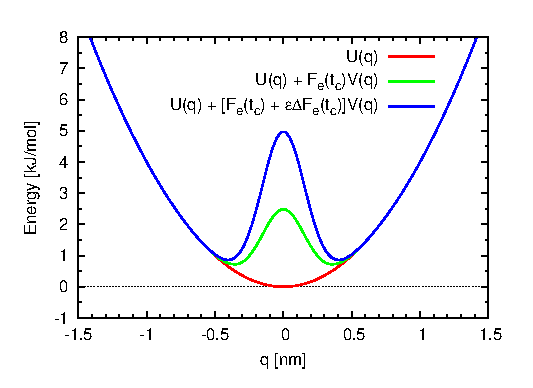
\includegraphics[width=0.4\textwidth]{figs/fig-split-pot.eps}
  \caption{The single-well potential with splitting perturbation.}
  \label{fig:tmp4}
\end{figure}

\begin{figure}
  \centering
  \includegraphics[width=0.95\textwidth]
  {figs/fig-split-str1-2d-more.eps}
  \caption{The plot of $\Delta\mt_\tau f(\vect x,t)$  under perturbation of
    $F_e^{\textrm{max}} = 1.0$.
    The 1st row: the direct non-equilibrium
    simulation. The 2nd row: the results of linear response
    formula~\eqref{eqn:core-identify-approx-2}.
    The 3rd row: the results of response
    formula~\eqref{eqn:pert-approx-1} and \eqref{eqn:pert-approx-2}.
    The order is 2, the reference state is $F_e^{\textrm{max}} = 0$, i.e.
    the equilibrium state.
  }
  \label{fig:tmp5}
\end{figure}

\begin{figure}
  \centering
  \includegraphics[width=0.95\textwidth]
  {figs/fig-split-str2-2d-more.eps}
  \caption{The plot of $\Delta\mt_\tau f(\vect x,t)$  under perturbation of
    $F_e^{\textrm{max}} = 2.0$.
    The 1st row: the direct non-equilibrium
    simulation. The 2nd row: the results of linear response
    formula~\eqref{eqn:core-identify-approx-2}.
    The 3rd row: the results of response
    formula~\eqref{eqn:pert-approx-1} and \eqref{eqn:pert-approx-2}.
    The order is 2, the reference state is $F_e^{\textrm{max}} = 0.0$, i.e.
    the equilibrium state.
    The 4th row: the results of response
    formula~\eqref{eqn:pert-approx-1} and \eqref{eqn:pert-approx-2}.
    The order is 1, the reference state is $F_e^{\textrm{max}} = 1.0$.
  }
  \label{fig:tmp6}
\end{figure}


In this splitting single-well potential example, the unperturbed
potential is simply the harmonic potential given by:
\begin{align}
  U(\vect q) = \frac12\,k\,\vect q^2 
\end{align}
Here $k = 8$~$\textsf{kJ} / (\textsf{mol nm}^2)$.
Notice at room temperature $300\ \textsf{K}$, $k_BT = 2.48$~\textsf{kJ/mol}.
See the red line in Fig.~\ref{fig:tmp4}.
%$\textsf{kJ} / (\textsf{mol nm}^4)}$
The perturbation is again given by
\begin{align}
  \vect C(\vect p, \vect q) = 0; \qquad
  \vect D(\vect p, \vect q) = -\nabla_{\vect q} V(\vect q) 
\end{align}
where $V(\vect q)$ is a Gaussian type potential:
\begin{align}
  V(\vect q) = \frac{1}{\sqrt{2\pi \sigma^2}}
  \exp\Big\{-\frac{\vect q^2}{2\sigma^2}\Big\}
\end{align}
we use $\sigma = 0.16$~\textsf{nm}. Please see Fig~\ref{fig:tmp4}.
For the results, please see Fig.~\ref{fig:tmp5} -- Fig.~\ref{fig:tmp6}.









\newpage
\section{Numerical results}
\subsection{Tilting double-well potential}

\begin{figure}
  \centering
  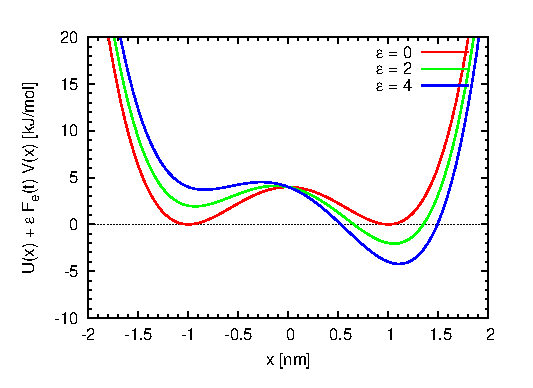
\includegraphics[width=0.4\textwidth]{figs/fig-tilt-pot.eps}
  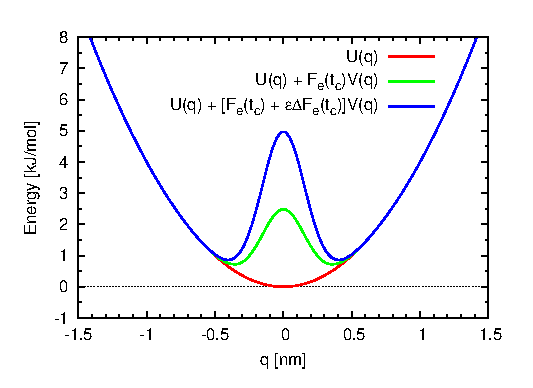
\includegraphics[width=0.4\textwidth]{figs/fig-split-pot.eps}
  \caption{Two testing cases presented by this paper.
    Left: the double-well potential with tilting perturbation.
    Right: the single-well potential with splitting perturbation.}
  \label{fig:new-tmp1}
\end{figure}


We test the idea by a one-dimensional model system: one particle in a
tilting double-well potential. For convenience, we let the mass of the
particle to be 1 \textsf{amu}. The unperturbed
Hamiltonian of the system is given by:
\begin{align}
  \mh (\vect p, \vect q) = \frac 12 \vect p^2 + U(\vect q) 
\end{align}
with potential
\begin{align}
  U(\vect q) = \frac12 k (\vect q^2 - a^2)^2
\end{align}
Here $k = 8$~$\textsf{kJ} / (\textsf{mol nm}^4)$, and $ a = 1\ \textsf{nm}$.
Notice at room temperature $300\ \textsf{K}$, $k_BT = 2.48$~\textsf{kJ/mol}.
See the red line in Fig.~\ref{fig:tmp1}.
%$\textsf{kJ} / (\textsf{mol nm}^4)}$
The perturbation is given by
\begin{align}
  \vect C(\vect p, \vect q) = 0; \qquad
  \vect D(\vect p, \vect q) = -\nabla_{\vect q} V(\vect q) = 1
\end{align}
Here $V(\vect q) = -\vect q$ is  effectively tilting the original
potential $U(\vect q)$. The strength of the perturbation $F_e(t)$ is given
by the following function:
\begin{align}
  F_e(t) = 
  \begin{cases}
    F_e^{\textrm{max}}\times (t / t_c) & t < t_c \\
    F_e^{\textrm{max}} & t \geq t_c
  \end{cases}
\end{align}
$t_c = 20$~\textsf{ps} so that the perturbation increases slow
enough: the typical decaying time scale of the correlation function
in~\eqref{eqn:core-identify-approx-2} is roughly 3~\textsf{ps}.
We choose $\tau = 1$~\textsf{ps}.
% We choose $\mt_\alpha$
% to be the propagator of the Langevin dynamics at temperature $150$
% \textsf{K} with $\alpha = 1$ \textsf{ps}.
Since the dynamics is in
1-d, the projection $\mathcal P$ is identity.  We consider the stability of the
distribution $f(\vect x, t)$ at time $t$: $\Delta\mt_\tau f(\vect x, t)$.
The larger
this value, the more stable the core sets are.

\begin{figure}
  \centering
  \includegraphics[width=0.95\textwidth]
  {figs/fig-tilt-str2-simple.eps}
  \caption{
    Tilting double well potential testing case:
    the plot of $\Delta\mt_\tau f(\vect x,t)$  under perturbation of
    $F_e^{\textrm{max}} = 2.0$.
    From left to right:
    (a) $t=0$~\textsf{ps},
    the brutal force non-equilibirum simulation,
    (b) $t=20$~\textsf{ps},
    the brutal force non-equilibirum simulation,
    (c) $t=20$~\textsf{ps},
    response formula truncated at order $n=1$,
    and
    (d) $t=20$~\textsf{ps},
    response formula truncated at order $n=2$.
    The equilibirum state serves as the reference of
    the response simulations.
  }
  \label{fig:new-tmp2}
\end{figure}


\begin{figure}
  \centering
  \includegraphics[width=0.95\textwidth]
  {figs/fig-tilt-str4-simple.eps}
  \caption{
    Tilting double well potential:
    the plot of $\Delta\mt_\tau f(\vect x,t)$  under perturbation of
    $F_e^{\textrm{max}} = 4.0$.
    From left to right:
    (a) $t=0$~\textsf{ps},
    the brutal force non-equilibirum simulation,
    (b) $t=20$~\textsf{ps},
    the brutal force non-equilibirum simulation,
    (c) $t=20$~\textsf{ps},
    response formula with reference process $F_e^{\max} = 0.0$
    (i.e. equilibirum simulation),
    and
    (d) $t=20$~\textsf{ps},
    response formula with reference process $F_e^{\max} = 2.0$.
    The response formula are truncated at order $n=1$.
  }
  \label{fig:new-tmp3}
\end{figure}



The Fig.~\ref{fig:new-tmp2} and \ref{fig:new-tmp3} present
the application of the response theory to
calculate core sets of the tilting double-well potential.
Fig.~\ref{fig:new-tmp2} presents
the snapshot at $t=20$~\textsf{ps}
of $\Delta\mt_\tau f(\vect x,t)$ under the maximum perturbation
strength $F_e^{\max} = 2.0$. Response formula truncated
at both order $n=1$ and $n=2$ are compared to 
the brutal force non-equilibirum simulation.
No obviously difference is shown. The second order response result
is slightly more precise than the first order one, but the
statistical error is also larger, which makes the profile noisy.
This figure tells us that
(1) the modeling error of the linear response (1st order) is
negligibly small; (2) the statistical error of numerically measuring the
linear response is also small.
Fig.~\ref{fig:new-tmp3} presents the $t=20$~\textsf{ps}
snapshots of $\Delta\mt_\tau f(\vect x,t)$
under a larger perturbations $F_e^{\max} = 4.0$.
The linear reponse using the equilibirum process as the reference
shows poor accuracy: the left well vanishes in this case,
while the linear response produces  artifical structures.
Since the profile is smooth, which indicates
the statistical error of calculating the linear term is small,
the deviation comes from the modellng error, namely the contribution
of higher order response terms.
By including the second order response term reduces the left
artifical core set, but also creates artifical finer grained
structures. The statistical accuracy is also worse than the linear response.
Plot (d) present the result of the linear response
formula using reference process $F_e^{\max} = 2.0$, which
is the process presented in Fig.~\ref{fig:new-tmp2}.
Much better modelling accuracy is achieved:
the left artifical core set disappear and the
statistical accuracy is also satisfactory.

% See Fig. \ref{fig:tmp2} and \ref{fig:tmp3} for numerical result.  Both
% the direct non-equilibrium simulation and the response
% approximations are presented. Time slices $t = 0$, 10, 15 and 20
% \textsf{ps} are shown.  When the perturbation is small,
% i.e. $F_e^{\textrm{max}} = 2$, the direct non-equilibrium simulation
% and the linear response results are accurately consistent.
% The 2nd order response formula~\eqref{eqn:pert-approx-1} and
% \eqref{eqn:pert-approx-2} are even better, but the numerical error
% is bigger.
% As the
% perturbation grows stronger, the left well becomes less stable, while
% the right well becomes more stable.  When the perturbation is big,
% i.e. $F_e^{\textrm{max}} = 4$, the linear response result is no
% longer precise.
% When $t\geq 20$ \textsf{ps}, the left well basically
% disappears, however, the linear response calculation presents
% artifical occilation at the right well.
% The 2nd order response also has artifical effect, and the numerical
% uncertainty is high.
% The 4th rwo of Fig.~\ref{fig:tmp3} presents the 1st order result of the
% response formula~\eqref{eqn:pert-approx-1} and
% \eqref{eqn:pert-approx-2}, with
% respect to the reference state $F_e^{\textrm{max}} = 2$. The result
% is impressively improved compared with the linear response with respect to the
% equilibrium state.




\subsection{Splitting single-well potential}

In this splitting single-well potential example, the unperturbed
potential is simply the harmonic potential given by:
\begin{align}
  U(\vect q) = \frac12\,k\,\vect q^2 
\end{align}
Here $k = 8$~$\textsf{kJ} / (\textsf{mol nm}^2)$.
Notice at room temperature $300\ \textsf{K}$, $k_BT = 2.48$~\textsf{kJ/mol}.
See the red line in Fig.~\ref{fig:tmp4}.
%$\textsf{kJ} / (\textsf{mol nm}^4)}$
The perturbation is again given by
\begin{align}
  \vect C(\vect p, \vect q) = 0; \qquad
  \vect D(\vect p, \vect q) = -\nabla_{\vect q} V(\vect q) 
\end{align}
where $V(\vect q)$ is a Gaussian type potential:
\begin{align}
  V(\vect q) = \frac{1}{\sqrt{2\pi \sigma^2}}
  \exp\Big\{-\frac{\vect q^2}{2\sigma^2}\Big\}
\end{align}
we use $\sigma = 0.16$~\textsf{nm}. Please see Fig~\ref{fig:tmp4}.
For the results, please see Fig.~\ref{fig:tmp5} -- Fig.~\ref{fig:tmp6}.




\begin{figure}
  \centering
  \includegraphics[width=0.95\textwidth]
  {figs/fig-split-str1-simple.eps}
  \caption{
    Splitting single-well potential testing case:
    the plot of $\Delta\mt_\tau f(\vect x,t)$  under perturbation of
    $F_e^{\textrm{max}} = 1.0$.
    From left to right:
    (a) $t=0$~\textsf{ps},
    the brutal force non-equilibirum simulation,
    (b) $t=20$~\textsf{ps},
    the brutal force non-equilibirum simulation,
    (c) $t=20$~\textsf{ps},
    response formula truncated at order $n=1$,
    and
    (d) $t=20$~\textsf{ps},
    response formula truncated at order $n=2$.
    The equilibirum state serves as the reference of
    the response simulations.
  }
  \label{fig:new-tmp5}
\end{figure}


\begin{figure}
  \centering
  \includegraphics[width=0.95\textwidth]
  {figs/fig-split-str2-simple.eps}
  \caption{
    splitting single well potential:
    the plot of $\Delta\mt_\tau f(\vect x,t)$  under perturbation of
    $F_e^{\textrm{max}} = 2.0$.
    From left to right:
    (a) $t=0$~\textsf{ps},
    the brutal force non-equilibirum simulation,
    (b) $t=20$~\textsf{ps},
    the brutal force non-equilibirum simulation,
    (c) $t=20$~\textsf{ps},
    response formula with reference process $F_e^{\max} = 0.0$
    (i.e. equilibirum simulation),
    and
    (d) $t=20$~\textsf{ps},
    response formula with reference process $F_e^{\max} = 1.0$.
    The response formula are truncated at order $n=1$.
  }
  \label{fig:new-tmp6}
\end{figure}







\section*{References}
\bibliography{ref}{}
\bibliographystyle{unsrt}





\end{document}